% Options for packages loaded elsewhere
\PassOptionsToPackage{unicode}{hyperref}
\PassOptionsToPackage{hyphens}{url}
%
\documentclass[
  12pt,
]{article}
\title{Air Quality Analysis of Fifteen Counties in North Carolina
(2018-2019)}
\usepackage{etoolbox}
\makeatletter
\providecommand{\subtitle}[1]{% add subtitle to \maketitle
  \apptocmd{\@title}{\par {\large #1 \par}}{}{}
}
\makeatother
\subtitle{\url{https://github.com/domeyerd/Domeyer_ENV872_EDA_FinalProject}}
\author{Devin Domeyer}
\date{}

\usepackage{amsmath,amssymb}
\usepackage{lmodern}
\usepackage{iftex}
\ifPDFTeX
  \usepackage[T1]{fontenc}
  \usepackage[utf8]{inputenc}
  \usepackage{textcomp} % provide euro and other symbols
\else % if luatex or xetex
  \usepackage{unicode-math}
  \defaultfontfeatures{Scale=MatchLowercase}
  \defaultfontfeatures[\rmfamily]{Ligatures=TeX,Scale=1}
  \setmainfont[]{Times New Roman}
\fi
% Use upquote if available, for straight quotes in verbatim environments
\IfFileExists{upquote.sty}{\usepackage{upquote}}{}
\IfFileExists{microtype.sty}{% use microtype if available
  \usepackage[]{microtype}
  \UseMicrotypeSet[protrusion]{basicmath} % disable protrusion for tt fonts
}{}
\makeatletter
\@ifundefined{KOMAClassName}{% if non-KOMA class
  \IfFileExists{parskip.sty}{%
    \usepackage{parskip}
  }{% else
    \setlength{\parindent}{0pt}
    \setlength{\parskip}{6pt plus 2pt minus 1pt}}
}{% if KOMA class
  \KOMAoptions{parskip=half}}
\makeatother
\usepackage{xcolor}
\IfFileExists{xurl.sty}{\usepackage{xurl}}{} % add URL line breaks if available
\IfFileExists{bookmark.sty}{\usepackage{bookmark}}{\usepackage{hyperref}}
\hypersetup{
  pdftitle={Air Quality Analysis of Fifteen Counties in North Carolina (2018-2019)},
  pdfauthor={Devin Domeyer},
  hidelinks,
  pdfcreator={LaTeX via pandoc}}
\urlstyle{same} % disable monospaced font for URLs
\usepackage[margin=2.54cm]{geometry}
\usepackage{longtable,booktabs,array}
\usepackage{calc} % for calculating minipage widths
% Correct order of tables after \paragraph or \subparagraph
\usepackage{etoolbox}
\makeatletter
\patchcmd\longtable{\par}{\if@noskipsec\mbox{}\fi\par}{}{}
\makeatother
% Allow footnotes in longtable head/foot
\IfFileExists{footnotehyper.sty}{\usepackage{footnotehyper}}{\usepackage{footnote}}
\makesavenoteenv{longtable}
\usepackage{graphicx}
\makeatletter
\def\maxwidth{\ifdim\Gin@nat@width>\linewidth\linewidth\else\Gin@nat@width\fi}
\def\maxheight{\ifdim\Gin@nat@height>\textheight\textheight\else\Gin@nat@height\fi}
\makeatother
% Scale images if necessary, so that they will not overflow the page
% margins by default, and it is still possible to overwrite the defaults
% using explicit options in \includegraphics[width, height, ...]{}
\setkeys{Gin}{width=\maxwidth,height=\maxheight,keepaspectratio}
% Set default figure placement to htbp
\makeatletter
\def\fps@figure{htbp}
\makeatother
\setlength{\emergencystretch}{3em} % prevent overfull lines
\providecommand{\tightlist}{%
  \setlength{\itemsep}{0pt}\setlength{\parskip}{0pt}}
\setcounter{secnumdepth}{5}
\ifLuaTeX
  \usepackage{selnolig}  % disable illegal ligatures
\fi

\begin{document}
\maketitle

\newpage
\tableofcontents 
\newpage
\listoftables 
\newpage
\listoffigures 
\newpage

\hypertarget{rationale-and-research-questions}{%
\section{Rationale and Research
Questions}\label{rationale-and-research-questions}}

Communities in North Carolina are expanding. According to the latest
population estimate from the U.S. Census Bureau, 112,000 people settled
in the state in one year. As more people choose to make North Carolina
their home, understanding trends in air quality could greatly impact
what county is best for those with, for example, children or health
problems. Additionally, trends in the time of year these air pollutants
are most concentrated is useful for determining factors like when or
when not to be in the state if opportunity allows.

Ozone is a potent pollutant. According to the U.S. Environmental
Protection Agency (EPA), children are at the greatest risk of exposure
to ozone given its affect on lungs and aggravation of asthma attacks.
Older adults and those with respiratory illnesses are also at risk of
more severe side effects from ozone pollution, including lung
inflamation and aggravated lung diseases like emphysema and chronic
bronchitis.

The EPA warns that fine particulate matter pollution is another risk for
children, older adults and those with lung diseases as it can cause
aggravated asthma, heart attacks, decreased lung function, and general
difficulty breathing.

Daily monitoring data for seven different air pollutants are made
publicly available by the EPA in their Outdoor Air Quality Data portal.
For this study, ozone and PM2.5 (fine particulate matter) are analyzed
across all months of the years 2018 and 2019 in fifteen counties in
North Carolina to compare trends.

Research questions include:

\begin{enumerate}
\def\labelenumi{\arabic{enumi}.}
\item
  Is the air quality index for Ozone and PM2.5 significantly worse in
  the summer (June - August) compared to the rest of the year?
\item
  What county has the highest average Ozone and PM2.5 levels?
\end{enumerate}

\newpage

\hypertarget{dataset-information}{%
\section{Dataset Information}\label{dataset-information}}

\hypertarget{data-retrieval}{%
\subsection{Data Retrieval}\label{data-retrieval}}

Data was collected from the EPA's ``Outdoor Air Quality''Air Data''
program, which posts daily air quality data for public access. The data
for this project was pulled from outdoor monitors across the state of
North Carolina and retrieved using the ``download daily data'' query
with settings for pollutant type, year, and geography. All monitor sites
with data that met these parameters were downloaded. Four different
CSVs, ozone and PM2.5 for 2018 and 2019, were added to the project
repository for further analysis and can be retrieved from the GitHub
repository.

~~~~~~~~~~~~~~~~~~~~~~~~~~~~~~~~~Table 1: Information about the data
source.

\begin{longtable}[]{@{}
  >{\raggedright\arraybackslash}p{(\columnwidth - 2\tabcolsep) * \real{0.48}}
  >{\raggedright\arraybackslash}p{(\columnwidth - 2\tabcolsep) * \real{0.52}}@{}}
\toprule
\begin{minipage}[b]{\linewidth}\raggedright
Detail
\end{minipage} & \begin{minipage}[b]{\linewidth}\raggedright
Description
\end{minipage} \\
\midrule
\endhead
Data Source & EPA Outdoor Air Quality Data \\
Variables Used & Month, Air Quality Index (AQS), County, Latitude,
Longitude \\
Date Range & 2018 - 2019 \\
\bottomrule
\end{longtable}

\hypertarget{data-wrangling}{%
\subsection{Data Wrangling}\label{data-wrangling}}

Not all variables in the downloaded datasets were necessary for
analysis. The data wrangling began by subsetting the date, daily air
quality index, pollutant type, site name, and location for each
pollutant in each year. Using the ``intersect'' function, counties
included in all four dataframes were identified (Figure 1), and this
subset was combined into a single dataframe. A date columns specifying
month and year was added. Then, using the split-apply-combine approach,
the average air quality parameter was identified for each pollutant, for
each month, and in each county. Average month and county values for
ozone and PM2.5 are shown in Tables 2 and 3.

\begin{figure}
\centering
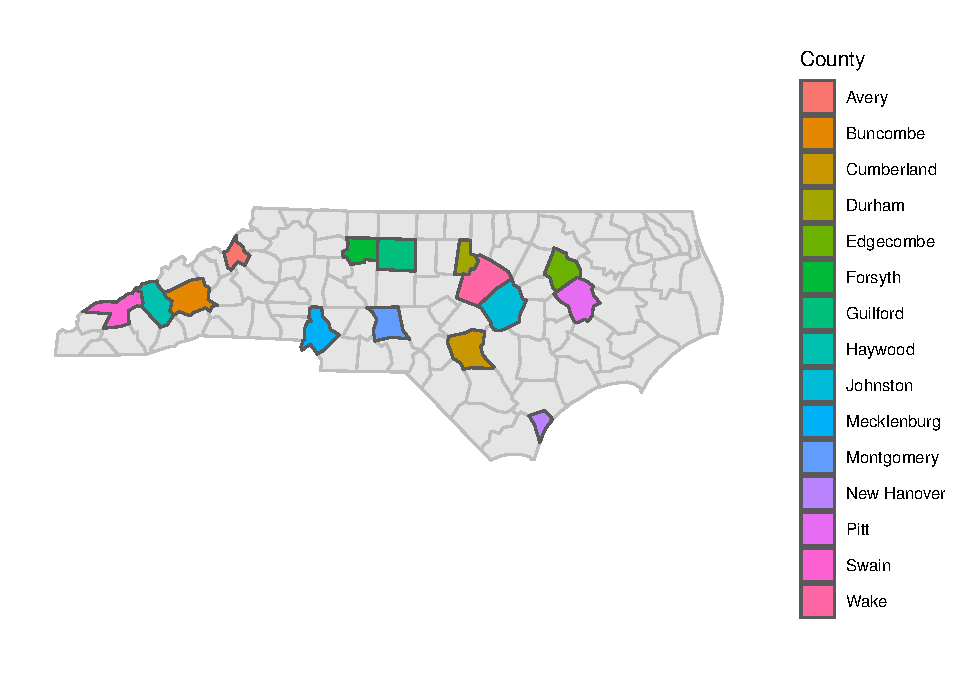
\includegraphics{Domeyer_FinalEDA_Sp22_files/figure-latex/geography-1.pdf}
\caption{Fifteen counties in North Carolina analyzed for this study}
\end{figure}

\begin{longtable}[]{@{}lrrrr@{}}
\caption{County summary of pollutants (ppm) in North Carolina, 2018 -
2019}\tabularnewline
\toprule
County & Mean\_Ozone & SD\_Ozone & Mean\_PM2.5 & SD\_PM2.5 \\
\midrule
\endfirsthead
\toprule
County & Mean\_Ozone & SD\_Ozone & Mean\_PM2.5 & SD\_PM2.5 \\
\midrule
\endhead
Avery & 38.61985 & 5.227705 & 19.07738 & 6.664508 \\
Buncombe & 39.11131 & 4.932966 & 25.82388 & 5.490064 \\
Cumberland & 41.62246 & 4.836873 & 29.83557 & 3.843253 \\
Durham & 39.57442 & 5.157252 & 33.41470 & 3.647563 \\
Edgecombe & 38.60864 & 4.763733 & 26.17416 & 7.099504 \\
Forsyth & 42.21695 & 6.356658 & 34.53112 & 2.852805 \\
Guilford & 45.16958 & 4.852739 & 29.15003 & 3.537174 \\
Haywood & 41.69665 & 4.870411 & 14.76863 & 7.788538 \\
Johnston & 39.51519 & 5.217194 & 33.07770 & 4.584117 \\
Mecklenburg & 40.53565 & 10.491038 & 35.05731 & 3.010584 \\
Montgomery & 35.72132 & 5.479213 & 30.00906 & 2.650936 \\
New Hanover & 38.45720 & 4.963110 & 15.26131 & 3.553639 \\
Pitt & 40.54210 & 5.587214 & 27.34060 & 4.781591 \\
Swain & 35.62953 & 5.724434 & 30.58757 & 2.999919 \\
Wake & 38.45918 & 8.125071 & 35.86295 & 2.723970 \\
\bottomrule
\end{longtable}

\begin{longtable}[]{@{}rrrrr@{}}
\caption{Monthly summary of pollutants (ppm) in North Carolina, 2018 -
2019}\tabularnewline
\toprule
Month & Mean\_Ozone & SD\_Ozone & Mean\_PM2.5 & SD\_PM2.5 \\
\midrule
\endfirsthead
\toprule
Month & Mean\_Ozone & SD\_Ozone & Mean\_PM2.5 & SD\_PM2.5 \\
\midrule
\endhead
1 & 33.32619 & 3.546046 & 25.62459 & 9.568661 \\
2 & 35.31075 & 3.259475 & 25.00483 & 8.674963 \\
3 & 42.68370 & 1.571070 & 26.52418 & 6.480162 \\
4 & 47.16908 & 1.894214 & 26.12349 & 6.489798 \\
5 & 43.69714 & 3.116447 & 30.51031 & 5.988857 \\
6 & 45.48342 & 4.349641 & 33.11955 & 5.685688 \\
7 & 42.01076 & 5.259302 & 33.83696 & 6.008032 \\
8 & 38.39003 & 5.251806 & 31.48924 & 5.102503 \\
9 & 37.33281 & 4.535845 & 29.43493 & 8.648364 \\
10 & 33.90310 & 1.656982 & 23.10596 & 6.735009 \\
11 & 29.67545 & 3.692872 & 26.19120 & 8.646493 \\
12 & 29.06040 & 5.240743 & 25.01234 & 9.391420 \\
\bottomrule
\end{longtable}

\newpage

\hypertarget{exploratory-analysis}{%
\section{Exploratory Analysis}\label{exploratory-analysis}}

It should be noted that there were some months in some counties that did
not have air quality indices for ozone or PM2.5 respectively. Air
quality readings can fluctuate quite drastically from month to month so
interpolated values were not added. Missing data was also concentrated
in the winter months which still enabled trend analysis for research
question one. Once the data was in a conducive format for analysis, it
was important to examine some initial visual trends. Average ozone
levels for each county are displayed in Figure 2, and average PM2.5
levels for each county are displayed in Figure 3 -- each for every month
of the year. From this initial visualization, patterns of potential
significance can be gleaned.

\begin{figure}
\centering
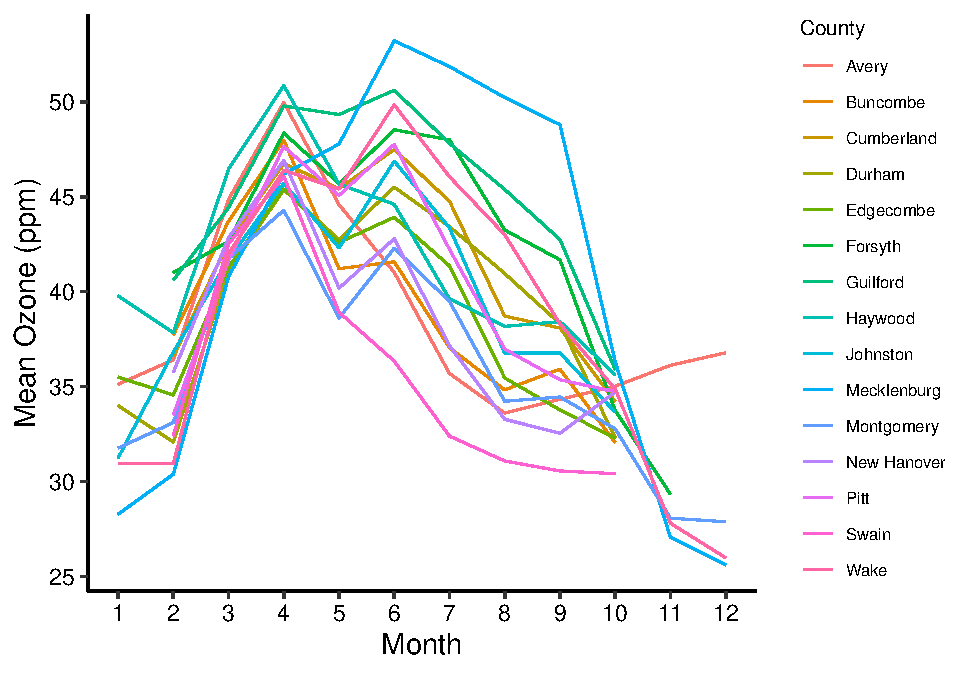
\includegraphics{Domeyer_FinalEDA_Sp22_files/figure-latex/exploration2-1.pdf}
\caption{Average ozone levels for each county across 2018 and 2019.}
\end{figure}

\begin{figure}
\centering
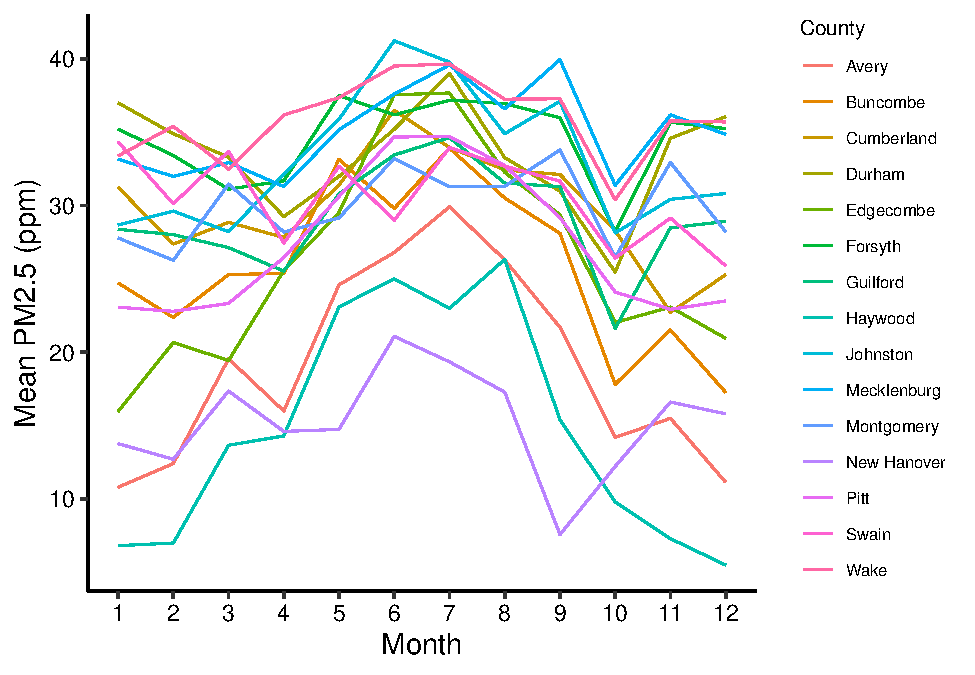
\includegraphics{Domeyer_FinalEDA_Sp22_files/figure-latex/exploration3-1.pdf}
\caption{Average fine particulate matter (PM2.5) levels for each county
across 2018 and 2019.}
\end{figure}

\newpage

\hypertarget{analysis}{%
\section{Analysis}\label{analysis}}

\hypertarget{question-1-is-the-air-quality-index-for-ozone-and-pm2.5-significantly-worse-in-the-summer-june---august-compared-to-the-rest-of-the-year}{%
\subsection{Question 1: Is the air quality index for Ozone and PM2.5
significantly worse in the summer (June - August) compared to the rest
of the
year?}\label{question-1-is-the-air-quality-index-for-ozone-and-pm2.5-significantly-worse-in-the-summer-june---august-compared-to-the-rest-of-the-year}}

To answer the first research question, a linear model was run with ozone
as the dependent variable and county and month as the independent
variables. A stepwise AIC analysis was conducted to determine the model
that explained the most variance in the data, and the result was
including only month as a factor to explain variation in ozone levels
fit the data best. A post-hoc Tukey HSD test revealed differences
between individual months. Ozone was significantly different across
months, with March-June significantly higher than October-February.
(ANOVA, df = 150, F = 15.19, p \textless{} 0.001) In contrast, month had
an almost non-existent effect on PM2.5 (p=0.99) and a stepwise AIC
confirmed that including only county to explain variation in the
dependent variable resulted in the best fitting model. Figure 4 shows
the contrast between monthly significance across both pollutants. It
should be noted that although month was the best fitting variable tested
in this study, it still only explained 8.6\% of the trend in the data.

\begin{figure}
\centering
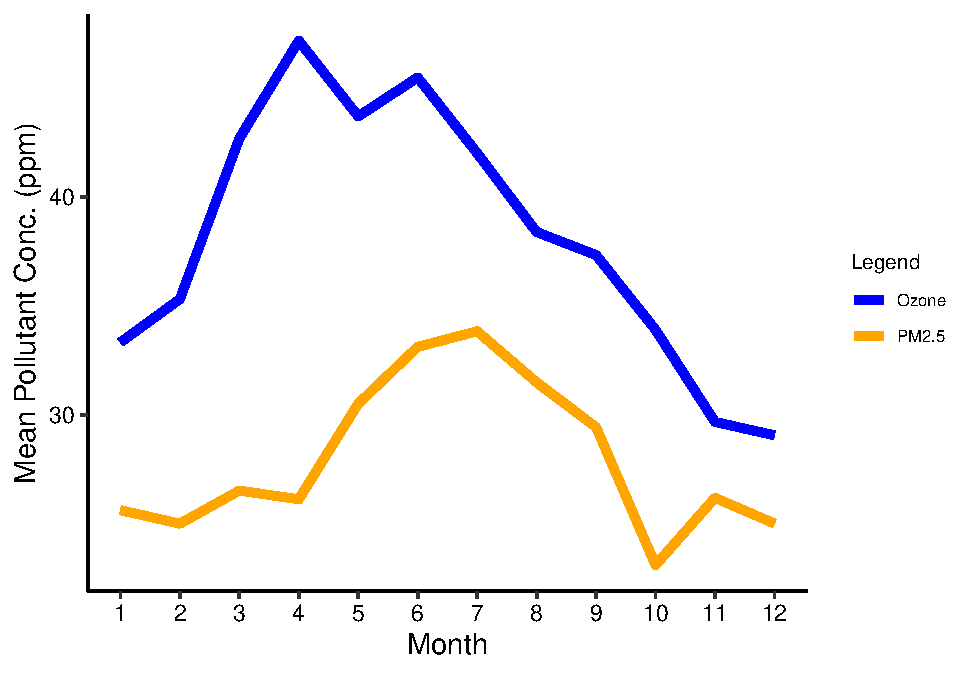
\includegraphics{Domeyer_FinalEDA_Sp22_files/figure-latex/results month-1.pdf}
\caption{Average monthly ozone and fine partciulate matter (PM2.5)
levels, aggregated across all fifteen counties in 2018 and 2019.}
\end{figure}

\hypertarget{question-2-what-county-has-the-highest-average-ozone-and-pm2.5-levels}{%
\subsection{Question 2: What county has the highest average Ozone and
PM2.5
levels?}\label{question-2-what-county-has-the-highest-average-ozone-and-pm2.5-levels}}

Given there was no significant difference in ozone levels across the
fifteen counties examined in this study, research question two goes, in
part, unanswered. However, PM2.5 was different across counties, with
Avery, New Hanover, and Haywood at significantly lower air quality index
levels than other counties. (ANOVA, df = 165, F= 25.86, p \textless{}
0.0001) This model fit significantly better than those run for research
question one, with change in county explaining 67\% of variation in
PM2.5 levels.

\begin{figure}
\centering
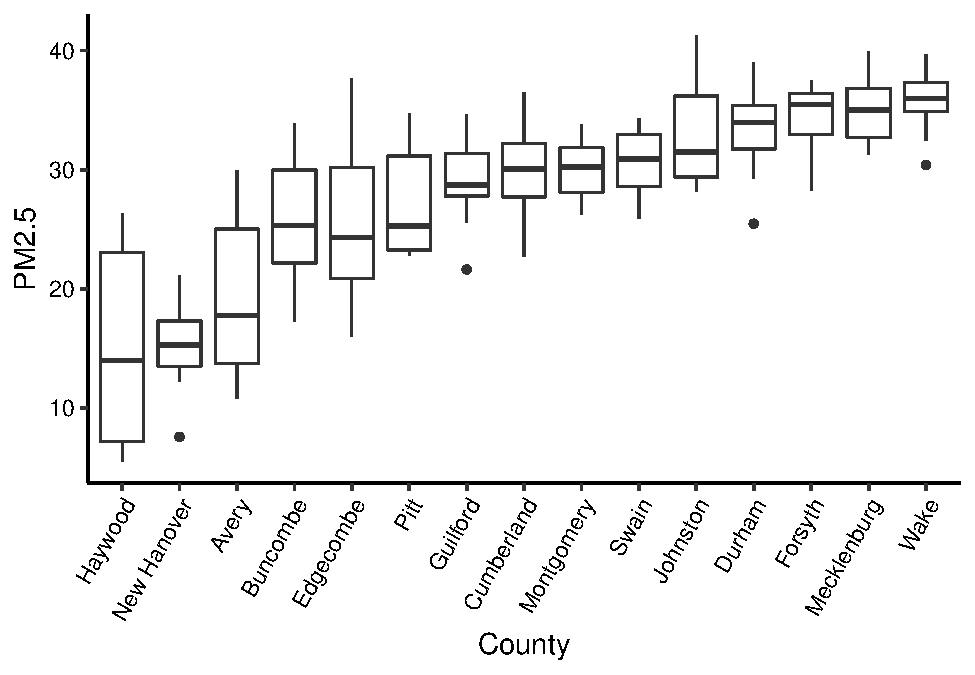
\includegraphics{Domeyer_FinalEDA_Sp22_files/figure-latex/results county-1.pdf}
\caption{Average yearly fine particulate matter (PM2.5) levels across
fifteen counties in 2018 and 2019.}
\end{figure}

\newpage

\hypertarget{summary-and-conclusions}{%
\section{Summary and Conclusions}\label{summary-and-conclusions}}

From this analysis, the increasing numbers of people moving to areas of
North Carolina should have more information on which counties would be
the safest for children, elderly or those with health concerns. That
said, this analysis only covers fifteen of the many counties in North
Carolina so further study would ne needed to make a final conclusion
about which county in North Carolina had the lowest levels of ozone or
fine particulate matter. Additionally, this study covered only data from
the years 2018 and 2019, which is now three years out of sync with
current air quality trends that can fluctuate dramatically, especially
in the era of extreme climate change.

For those looking to visit North Carolina or potentially make it their
second home, the summer months could be ones to avoid if there are those
traveling with health concerns, children or elderly. Although fine
particulate matter did not vary significantly between months of the
year, ozone levels were highest during the Spring months, tapering out
toward the end of summer. Ozone is still an aggravator of respiratory
problems including asthma so the insignificance of fine particulates
should not assuage seasonal health concerns.

\end{document}
